\documentclass[final]{beamer}

\usepackage[scale=1.24]{beamerposter} % Use the beamerposter package for laying out the poster

\usetheme{confposter} % Use the confposter theme supplied with this template

\setbeamercolor{block title}{fg=ngreen,bg=white} % Colors of the block titles
\setbeamercolor{block body}{fg=black,bg=dblue!10} % Colors of the body of blocks
\setbeamercolor{block alerted title}{fg=white,bg=dblue!70} % Colors of the highlighted block titles
\setbeamercolor{block alerted body}{fg=black,bg=dblue!10} % Colors of the body of highlighted blocks
% Many more colors are available for use in beamerthemeconfposter.sty

%-----------------------------------------------------------
% Define the column widths and overall poster size
% To set effective sepwid, onecolwid and twocolwid values, first choose how many columns you want and how much separation you want between columns
% In this template, the separation width chosen is 0.024 of the paper width and a 4-column layout
% onecolwid should therefore be (1-(# of columns+1)*sepwid)/# of columns e.g. (1-(4+1)*0.024)/4 = 0.22
% Set twocolwid to be (2*onecolwid)+sepwid = 0.464
% Set threecolwid to be (3*onecolwid)+2*sepwid = 0.708

\newlength{\sepwid}
\newlength{\onecolwid}
\newlength{\twocolwid}
\newlength{\threecolwid}
\setlength{\paperwidth}{48in} % A0 width: 46.8in
\setlength{\paperheight}{36in} % A0 height: 33.1in
\setlength{\sepwid}{0.024\paperwidth} % Separation width (white space) between columns
\setlength{\onecolwid}{0.22\paperwidth} % Width of one column
\setlength{\twocolwid}{0.464\paperwidth} % Width of two columns
\setlength{\threecolwid}{0.708\paperwidth} % Width of three columns
\setlength{\topmargin}{-0.5in} % Reduce the top margin size
%-----------------------------------------------------------

\usepackage{graphicx}  % Required for including images

\usepackage{booktabs} % Top and bottom rules for tables

\usepackage{hanging} % Used for hanging indents in the reference section

\usepackage{tikz} % Used for adding image to title

%----------------------------------------------------------------------------------------
%	TITLE SECTION 
%----------------------------------------------------------------------------------------

\title{\Huge\textbf{Using a Fitness Tracker to Predict Automatically Reinforced Problem Behavior}} % Poster title

\author{\huge Blake Crosby and Halie Tumbleston} % Author(s)

\institute{\huge ABX Solutions, LLC} % Institution(s)

%----------------------------------------------------------------------------------------

\begin{document}

\addtobeamertemplate{headline}{} 
{
	\begin{tikzpicture}[remember picture,overlay] 
		\node [shift={(6 cm,-5cm)}] at (current page.north west) {
\includegraphics[height=9cm]{abx_logo.jpg}}; 
	\end{tikzpicture} 
}

\addtobeamertemplate{headline}{} 
{
	\begin{tikzpicture}[remember picture,overlay] 
		\node [shift={(-6 cm,-5cm)}] at (current page.north east) {
\includegraphics[height=9cm]{qrcode.png}}; 
	\end{tikzpicture} 
}
\addtobeamertemplate{block end}{}{\vspace*{2ex}} % White space under blocks
\addtobeamertemplate{block alerted end}{}{\vspace*{2ex}} % White space under highlighted (alert) blocks

\setlength{\belowcaptionskip}{2ex} % White space under figures
\setlength\belowdisplayshortskip{2ex} % White space under equations

\begin{frame}[t] % The whole poster is enclosed in one beamer frame

\begin{columns}[t] % The whole poster consists of three major columns, the second of which is split into two columns twice - the [t] option aligns each column's content to the top

\begin{column}{\sepwid}\end{column} % Empty spacer column

\begin{column}{\onecolwid} % The first column

%----------------------------------------------------------------------------------------
%	INTRODUCTION
%----------------------------------------------------------------------------------------

\begin{alertblock}{Introduction}
	
	\begin{itemize}
		\item Smart watches have become ubiquitous in developed nations due to their falling cost and increased functionality
		\item Among their many uses, smart watches can serve as fitness trackers that monitor body temperature, heart rate (HR), muscle motion, and other health data (Lu et al., 2016)
		\item Automatically reinforced problem behaviors associated with heightened states of physical activity (e.g., self-injurious behavior) may correlate with increased HR
		\item Similarly, elevated HR could be predictive of problem behavior before it occurs
		\item If a relationship were established between elevated HR and problem behavior, then HR could potentially be used a cue to take action before the behavior begins
		
	\end{itemize}

\end{alertblock}

%----------------------------------------------------------------------------------------
%	METHOD
%----------------------------------------------------------------------------------------

\begin{alertblock}{Method}
	\begin{center}
		\textbf{Participants}
	\end{center}
	\begin{itemize}
		\item A fifteen year old male with autism who has a history of automatically reinforced problem behavior
		\item A Functional Behavior Assessment was conducted on the subject to rule out socially mediated reinforcement of problem behavior
	\end{itemize}

	\begin{center}
		\textbf{Targets}
	\end{center}
	\begin{itemize}
		\item \textit{Partial Overlap:} The percentage of problem behaviors where the reported time of the problem behavior partially overlapped with an elevated heart rate (HR > 100 bpm)
		\item \textit{Precedes Onset:} The percentage of problem behaviors where the reported time of the problem behavior was preceded by an elevated heart rate (HR > 100 bpm) by no more than 10 minutes
		\item 10 minutes was chosen to allow the increase in HR to potentially be connected to the problem behavior because not enough time would have elapsed for a cool-down period to occur
		\item Problem behavior was defined as self-injurious behavior (i.e., hand biting, striking the face with a closed fist, and head banging) and/or aggression towards others (i.e., attempts to bite, hit, or kick)
	\end{itemize}

	\begin{center}
		\textbf{Procedures}
	\end{center}
	\begin{itemize}
		\item An online form was created to collect information about each incidence of the subject's problem behavior from parents, teachers, and other caregivers
		\item HR information (i.e., bpm vs time) was collected from the Fitbit and downloaded into a spreadsheet
		\item The time and duration of each problem behavior was plotted to overlay time series data of the subject's HR to look for correlations between the two
		\item Information regarding the administration of emergency medication during problem behaviors was also recorded
	\end{itemize}

\end{alertblock}

%------------------------------------------------

\end{column} % End of the first column

\begin{column}{\sepwid}\end{column} % Empty spacer column

\begin{column}{\twocolwid} % Begin a column which is two columns wide (column 2)
	
%----------------------------------------------------------------------------------------
%	RESULTS
%----------------------------------------------------------------------------------------

\begin{alertblock}{Results}
	
	\begin{itemize}
		\item Data was collected for a ten week period from March 15 to May 24, 2018
		\item Below are examples of daily data collection showing heart rate versus time of day in blue
		\item Incidents of problem behavior are shown as red horizontal lines with the length corresponding to the duration of the episode
		\item These incidents are also annotated with text giving the onset time of the problem behavior followed by its duration
		\item A green star annotation was also used when the subject's emergency medication was administered
	\end{itemize}
	
\end{alertblock}

%----------------------------------------------------------------------------------------

\begin{columns}[t,totalwidth=\twocolwid] % Split up the two columns wide column

\begin{column}{\onecolwid}\vspace{-.6in} % The first column within column 2 (column 2.1)

%----------------------------------------------------------------------------------------
%	RESULTS
%----------------------------------------------------------------------------------------

%----------------------------------------------------------------------------------------
%	EXAMPLE 1
%----------------------------------------------------------------------------------------

\begin{block}{Example 1: Partial Overlap}
	
	\begin{figure}
		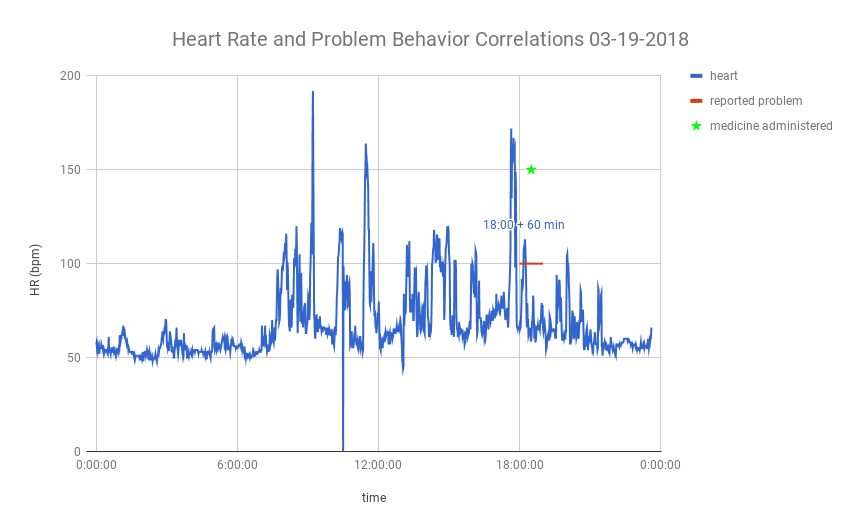
\includegraphics[width=0.8\linewidth]{Example1.png}
		\caption{Data collected on 3/19/2018 shows partial overlap of elevated HR and the reported time of the problem behavior. This was scored as a '1' for Partial Overlap and '0' for Precedes Onset.}
	\end{figure}
	
\end{block}

%----------------------------------------------------------------------------------------
%	EXAMPLE 2
%----------------------------------------------------------------------------------------

\begin{block}{Example 2: HR Elevation Precedes Onset}
	
	\begin{figure}
		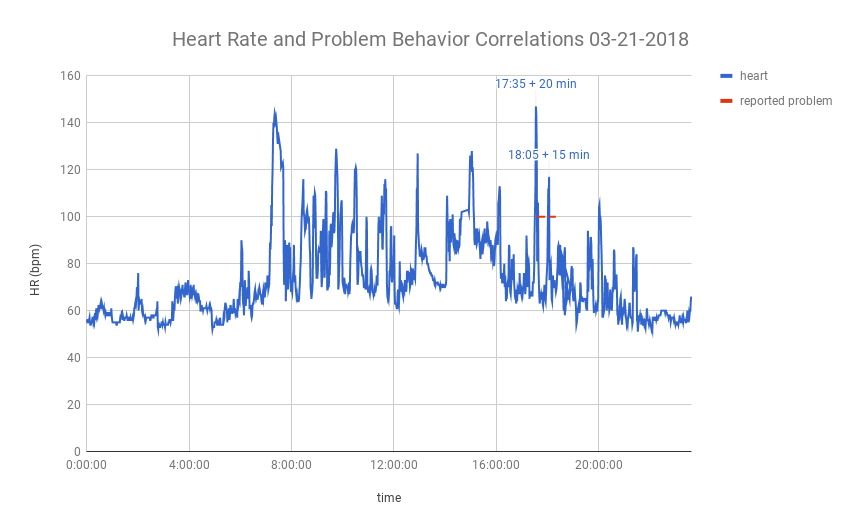
\includegraphics[width=0.8\linewidth]{Example2.png}
		\caption{Data collected on 3/21/2018 shows two incidents with elevated HR preceding the reported onset of the problem behavior. Both were scored as a '1' for Partial Overlap and '1' for Precedes Onset.}
	\end{figure}
	
\end{block}

%----------------------------------------------------------------------------------------
%	EXAMPLE 3
%----------------------------------------------------------------------------------------

\begin{block}{Example 3: HR Data Unavailable}
	
	\begin{figure}
		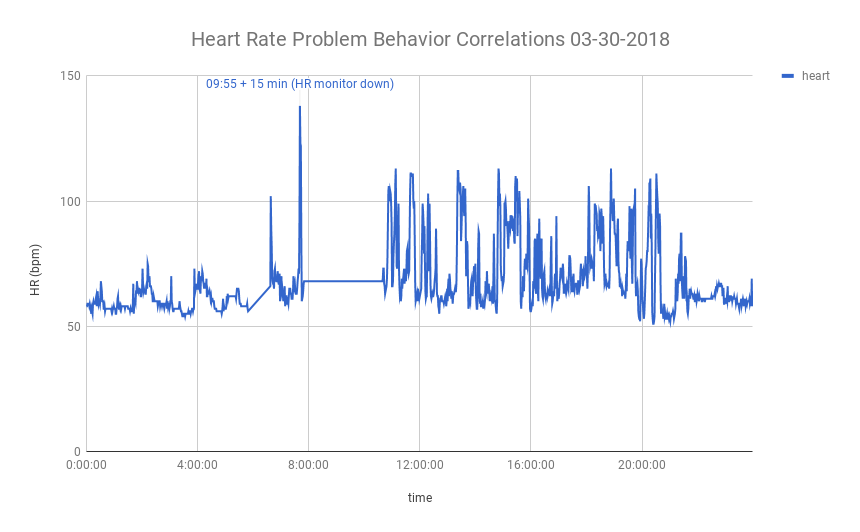
\includegraphics[width=0.8\linewidth]{Example3.png}
		\caption{Data collected on 3/30/2018 shows a problem behavior that occurred while the Fitbit charge was low and not collecting HR information. This data point was excluded from analysis.}
	\end{figure}
	
\end{block}


\end{column} % End of column 2.1

%----------------------------------------------------------------------------------------

\begin{column}{\onecolwid}\vspace{-.6in} % The second column within column 2 (column 2.2)

%----------------------------------------------------------------------------------------
%	EXAMPLE 4
%----------------------------------------------------------------------------------------

\begin{block}{Example 4: No Overlap}
	
	\begin{figure}
		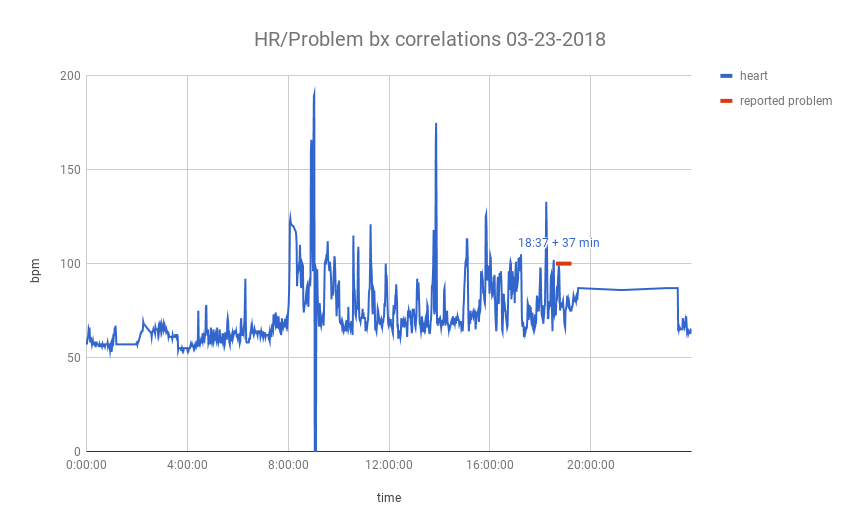
\includegraphics[width=0.8\linewidth]{Example4.png}
		\caption{Data collected on 4/25/2018 demonstrates a problem behavior that is not preceded by an elevated HR nor does it overlap with an elevated HR. This was scored as a '0' for Partial Overlap and '0' for Precedes Onset. }
	\end{figure}
	
\end{block}

%----------------------------------------------------------------------------------------
%	EXAMPLE 5
%----------------------------------------------------------------------------------------

\begin{block}{Example 5: HR Elevation Follows Onset}
	
	\begin{figure}
		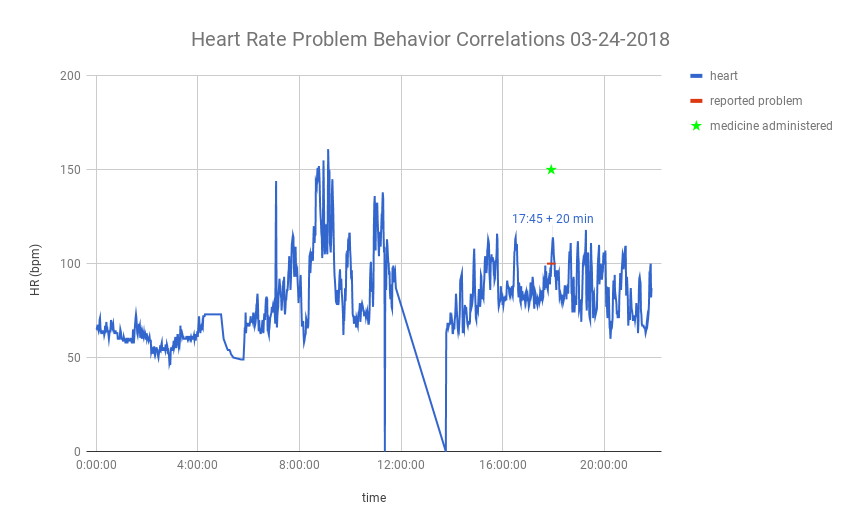
\includegraphics[width=0.8\linewidth]{Example5.png}
		\caption{Data collected on 3/24/2018 shows an elevated HR following the reported onset of problem behavior. This was scored as a '1' for Partial Overlap and '0' for Precedes Onset.}
	\end{figure}
	
\end{block}

%----------------------------------------------------------------------------------------
%	EXAMPLE 6
%----------------------------------------------------------------------------------------

\begin{block}{Example 6: Multiple Problem Behaviors}
	
	\begin{figure}
		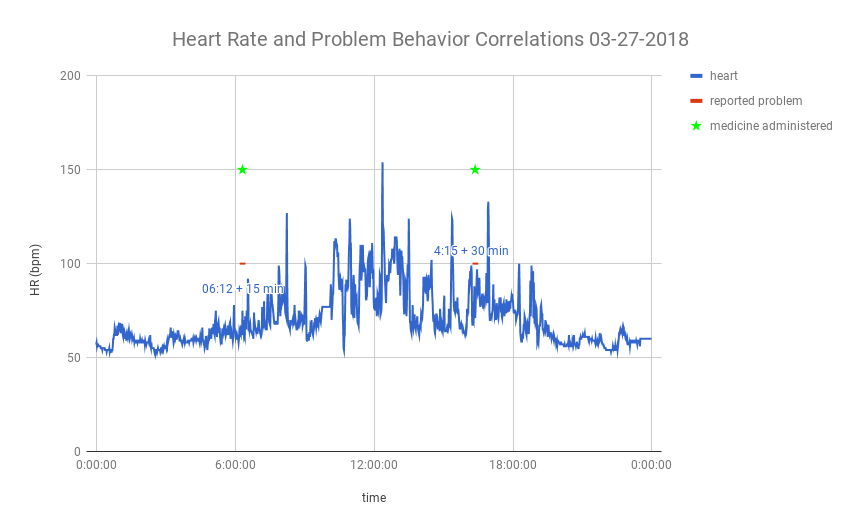
\includegraphics[width=0.8\linewidth]{Example6.png}
		\caption{Data collected on 3/27/2018 demonstrates multiple problem behaviors on one day. Each was scored separately.}
	\end{figure}
	
\end{block}


\end{column} % End of column 2.2

\end{columns} % End of the split of column 2 - any content after this will now take up 2 columns width


\begin{columns}[t,totalwidth=\twocolwid] % Split up the two columns wide column again

\begin{column}{\onecolwid} % The first column within column 2 (column 2.1)

%----------------------------------------------------------------------------------------

\end{column} % End of column 2.1

\begin{column}{\onecolwid} % The second column within column 2 (column 2.2)

%----------------------------------------------------------------------------------------

\end{column} % End of column 2.2

\end{columns} % End of the split of column 2

\end{column} % End of the second column

\begin{column}{\sepwid}\end{column} % Empty spacer column

\begin{column}{\onecolwid} % The third column

%----------------------------------------------------------------------------------------
%	RESULTS
%----------------------------------------------------------------------------------------

\begin{alertblock}{Results (continued)}
	
	\begin{center}
		\begin{tabular}{|c||c||c|} 
			\hline\hline
			Date & Partial Overlap & Precedes Onset\\
			\hline\hline
			3/19/2018 & 1 & 0\\
			\hline\hline
			3/21/2018 & 1 & 1\\
			\hline\hline
			3/21/2018 & 1 & 1\\
			\hline\hline
			3/23/2018 & 0 & 1\\
			\hline\hline
			3/24/2018 & 1 & 0\\
			\hline\hline
			3/27/2018 & 0 & 0\\
			\hline\hline
			3/27/2018 & 0 & 0\\
			\hline\hline
			3/28/2018 & 1 & 1\\
			\hline\hline
			%3/28/2018 & 1 & 0\\
			%\hline\hline
			%3/28/2018 & 0 & 0\\
			%\hline\hline
			%3/29/2018 & 0 & 0\\
			%\hline\hline
			%3/29/2018 & 0 & 0\\
			%\hline\hline
			%4/12/2018 & 1 & 1\\
			%\hline\hline
			%4/12/2018 & 1 & 0\\
			%\hline\hline
			%4/13/2018 & 1 & 1\\
			%\hline\hline
			%4/13/2018 & 1 & 1\\
			%\hline\hline
			%4/16/2018 & 1 & 0\\
			%\hline\hline
			%4/16/2018 & 1 & 0\\
			%\hline\hline
			%4/16/2018 & 0 & 0\\
			%\hline\hline
			%4/17/2018 & 0 & 0\\
			%\hline\hline
			%4/18/2018 & 1 & 0\\
			%\hline\hline
			\hline\hline
			... & ... & ...\\
			%\hline\hline
			%4/19/2018 & 1 & 1\\
			%\hline\hline
			%4/19/2018 & 1 & 1\\
			%\hline\hline
			%4/20/2018 & 1 & 1\\
			%\hline\hline
			%4/20/2018 & 1 & 1\\
			\hline\hline
			4/23/2018 & 1 & 0\\
			\hline\hline
			4/23/2018 & 1 & 1\\
			\hline\hline
			4/23/2018 & 1 & 1\\
			\hline\hline
			4/24/2018 & 1 & 1\\
			\hline\hline
			4/25/2018 & 0 & 0\\
			\hline\hline
			5/7/2018 & 0 & 0\\
			\hline\hline
			5/10/2018 & 0 & 1\\
			\hline\hline
			\textbf{Totals} & 21/32=65.6\% & 15/32=46.9\%\\
			\hline\hline
		\end{tabular}
	\end{center}

	\begin{itemize}
		\item The reported time period of a problem behavior overlapped with a HR greater than 100 bpm on 65.6\% of episodes
		\item A HR greater than 100 bpm preceded the reported onset of problem behavior on 46.9\% of episodes
		
	\end{itemize}
	
\end{alertblock}

%----------------------------------------------------------------------------------------
%	DISCUSSION
%----------------------------------------------------------------------------------------

\begin{alertblock}{Discussion}
	
	\begin{itemize}
		\item A strong relationship was not established between elevated HR and reported times of problem behavior
		\item The study suffered from problems with the Fitbit battery being low during problem behaviors
		\item There were also problems with the reliability of the reported onset/offset times (i.e., not reporting an accurate onset time due to dealing with the problem behavior itself)
		\item Allowing for a certain degree of error in reporting the onset time may also improve the relationship
		\item The HR criteria of 100 bpm is somewhat arbitrary and adjusting this value may yield better results
		\item Future studies could determine if a self-monitoring intervention could help caregivers implement antecedent strategies to deter potential problem behaviors before they arise
	\end{itemize}
	
\end{alertblock}

%----------------------------------------------------------------------------------------

%----------------------------------------------------------------------------------------
%	REFERENCES
%----------------------------------------------------------------------------------------

\begin{alertblock}{References}
	
	\begin{hangparas}{.5in}{1}
		
		Lu, T. et al. (2016), Healthcare Applications of Smart Watches. \textit{Applied Clinical Informatics, 7}(3), 850-869
		
	\end{hangparas}
	
\end{alertblock}

%----------------------------------------------------------------------------------------
\setbeamercolor{block alerted title}{fg=black,bg=norange} % Change the alert block title colors
\setbeamercolor{block alerted body}{fg=black,bg=white} % Change the alert block body colors

\begin{alertblock}{For more information contact Blake Crosby}

\begin{itemize}
	\item ptsouth97@gmail.com
	\item https://github.com/ptsouth97/FitnessTracker
\end{itemize}

\end{alertblock}


%----------------------------------------------------------------------------------------

\end{column} % End of the third column

\end{columns} % End of all the columns in the poster

\end{frame} % End of the enclosing frame

\end{document}